% Created 2018-03-06 火 12:42
\documentclass[compress,dvipdfmx,xcolor=table]{beamer}
                                \newcommand{\latex}[1]{#1}
\newcommand{\st}[1]{\structure{#1}}
\newcommand{\stt}[1]{\structure{\texttt{#1}}}
\newcommand{\at}[1]{\alert{\texttt{#1}}}
\newcommand{\al}[1]{\alert{#1}}
\institute{$^{1}$Kobe University, Japan \and $^{2}$CRIL-CNRS UMR 8188, France}
\usepackage{multirow}
\usepackage{alltt}
\usepackage{amsmath}
\usepackage{tabularx}
\usepackage{tikz}
\usepackage{pifont}
\usetikzlibrary{shapes,arrows,calc,arrows.meta,}
\tikzstyle{block}=[draw opacity=0.7,line width=1.4cm]
\usetikzlibrary{patterns}
\usepackage{satmo}
\usepackage{array}
\renewcommand{\familydefault}{\sfdefault}
\usefonttheme[onlymath]{serif}
\usefonttheme{structurebold}
\usetheme{Boadilla}
\usecolortheme{orchid}
\usecolortheme{whale}
\setbeamertemplate{footline}{}
\setbeamertemplate{footline}[frame number]{}
\setbeamertemplate{navigation symbols}{}
\definecolor{nColor1}{rgb}{0.96,0.85,0.87}
\definecolor{grays}{rgb}{0.9,0.9,0.9}
\usepackage{appendixnumberbeamer}
\newcommand{\vr}{\vrule}
\newcommand{\en}{\vrule depth 0.4pt \vrule height 0em width 0.5em depth 0.4pt}
\newtheorem{property}{Property}
\newtheorem{proposition}{Proposition}
\usepackage{colortbl}
\newcommand{\OK}{\mbox{\textcolor{green}{\Pisymbol{pzd}{52}}}}
\newcommand{\KO}{\mbox{\textcolor{red}{\Pisymbol{pzd}{56}}}}
\usepackage{ulem}
\newcommand{\ctext}[1]{\raise0.2ex\hbox{\textcircled{\scriptsize{#1}}}}
\renewcommand{\maketitle}{}
\usetheme{default}
\author{Takehide Soh\inst{1}}
\date{Introduction of Scala Programming Language \newline March, 6th}
\title{Self Introduction}
\begin{document}

\maketitle

\section{}
\label{sec:orgheadline6}
\begin{frame}[label={sec:orgheadline1}]{Access the Lecture Home Page!}
\begin{itemize}
\item \url{http://kix.istc.kobe-u.ac.jp/~soh/cril-scala/}
\end{itemize}
\end{frame}

\begin{frame}[label={sec:orgheadline2}]{Lecturer}
\begin{itemize}
\item Takehide Soh
\item I have been working in Kobe University, Japan.
\item My research interest is constraint programming, a subject in AI.
\item I come to France and live in Lille with my family (wife and 2-ans
daughter) since last September as sabbatical.
\end{itemize}
\end{frame}

\begin{frame}[label={sec:orgheadline3}]{Japan?}
\begin{center}
\includegraphics[width=\hsize]{./figs/world-00.eps}\\
From Japan to France, it takes 12 hours by plains!
\end{center}
\end{frame}

\begin{frame}[label={sec:orgheadline4}]{Kobe?}
\begin{center}
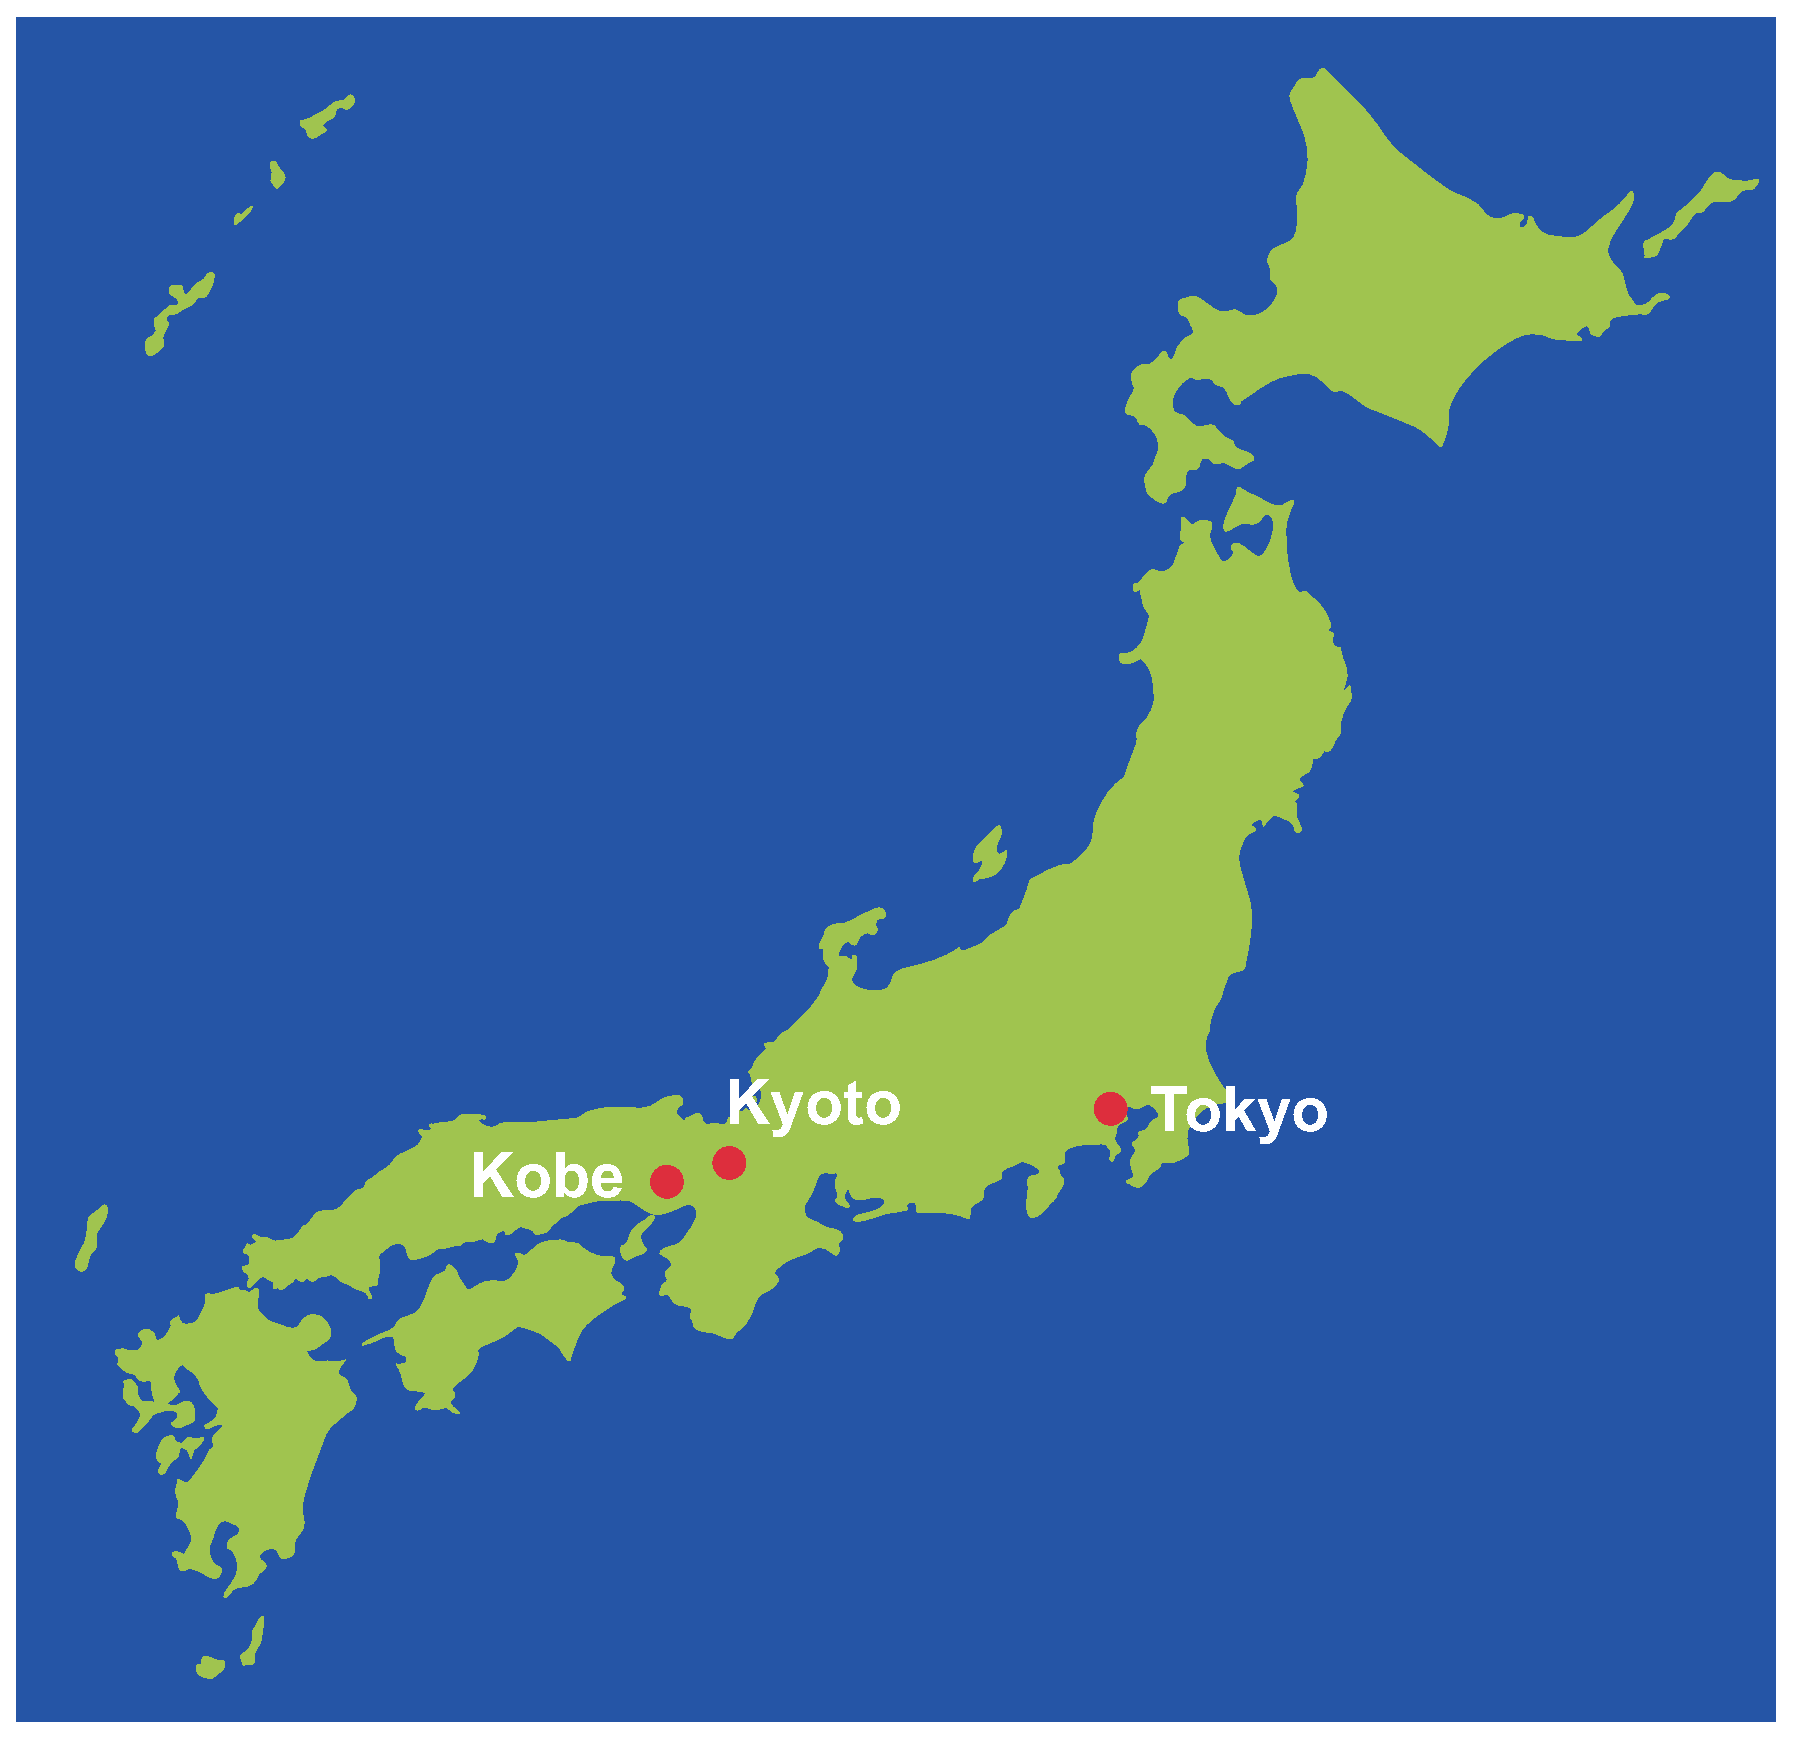
\includegraphics[width=0.65\hsize]{./figs/japan-00.eps}
\end{center}
\end{frame}

\begin{frame}[label={sec:orgheadline5}]{All French I can Speak!}
\begin{itemize}[<+->]
\item Ceci s'il vous plaît.
\item C'est tout.
\item C'est bon.
\item Très bien!
\item Oui. Non.
\item Bonjour! Bonsoir! Au revoir!
\item Merci!
\item Merci beaucoup!
\end{itemize}

\pause
I keep to train myself. So, please let me know other useful sentences
of French language.
\end{frame}
\end{document}
